\subsection{Backpropagation}

\begin{frame}
\frametitle{Notation}

\begin{figure}
	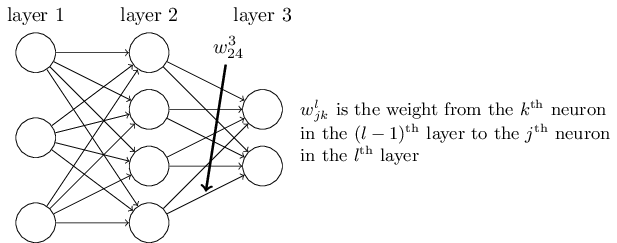
\includegraphics[width=\linewidth]{./geschichtliches/backpropagation/img/weight_notation}
\end{figure}

\note[item]{l: Exponent, steht für die Schicht
\begin{itemize}
    \item l - 1, weil man stets von hinten nach vorne schaut
\end{itemize}}

\note[item]{Eingabe wird auch als eigene Schicht verstanden}
\note[item]{j: Index Zielneuron}
\note[item]{k: Index Startneuron}

\end{frame}

\begin{frame}
\frametitle{Notation}

\begin{figure}
	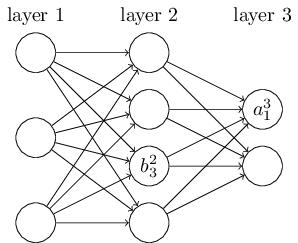
\includegraphics[width=.6\linewidth]{./geschichtliches/backpropagation/img/biasAct_notation}
\end{figure}

\begin{columns}

\column{.5\textwidth}
\begin{align*}
a^{l}_j = \sigma\left( \sum_k w^{l}_{jk} a^{l-1}_k + b^l_j \right) \Rightarrow 
\quad
\!
\begin{aligned}
a^l & = \sigma(z^l) \\
z^l & = w^l a^{l-1}+b^l \\
\end{aligned}
\end{align*}


\note[item]{Ähnlich zu Gewichtsnotation
\begin{itemize}
    \item l bezieht sich hierbei jedoch auf aktuelle Schicht
    \item j wie gehabt Index in Schicht
    \item Notation gilt auch für Aktivierung a
\end{itemize}}

\note[item]{Wichtig: $\sigma$ bezieht sich auf Vektor $\Rightarrow$ Vektorielle Funktion}
\note[item]{Jede Komponente einzeln mit $\sigma$ verarbeitet}
\note[item]{Abstraktion vom Ausgabewert vor der Aktivierungsfkt
\begin{itemize}
    \item hilft später beim Ableiten
\end{itemize}}

\hspace{10mm}

\end{columns}

\end{frame}



\begin{frame}
\frametitle{Backpropagation}

\begin{itemize}
\item{Kostenfunktion soll minimiert werden}
\item{Ziel: Optimale Gewichte und Schwellwerte finden}
\end{itemize}

\begin{itemize}
\item Grobe Vorgehensweise: Iterativer Prozess

\begin{itemize}	
	\item Fehlervektor der letzten Schicht berechnen
	\item Fehler schichtweise zum Eingabelayer zurückführen
	\item Parameter schichtweise nach Gradienten angleichen
\end{itemize}

\end{itemize}


\note[item]{1970er entwickelt, 1986 von Rummelhart, Hilten und Williams in Paper bekannt gemacht}
\note[item]{Kostenfunktion wie bei Gradientenabstieg / Adeline
\begin{itemize}
    \item Unterschied: Hier mehrschichtiges Netz
    \item Gradientenabstieg grob erläutert, ausgeblieben -
    \begin{itemize}
        \item Anwendung im mehrschichtigen Netz und mehrdimensionale Kostenfunktion
    \end{itemize}
\end{itemize}}

\note[item]{Fehlervektor der letzten Schicht berechnen
\begin{itemize}
    \item Fehler schichtweise zum Eingabelayer zurückführen
\end{itemize}}

\note[item]{Parameter schichtweise nach Gradienten angleichen}

\end{frame}


\begin{frame}
\frametitle{Fehler - Ausgabeschicht} 

\begin{columns}

\begin{column}{0.5\textwidth}
\myeq{
\delta^L_j & = \frac{\partial C}{\partial z^L_j} \\
 & = \sum_k \frac{\partial C}{\partial a^L_k} \frac{\partial a^L_k}{\partial z^L_j} \\
 & = \frac{\partial C}{\partial a^L_j} \frac{\partial a^L_j}{\partial z^L_j} \\
 & = \frac{\partial C}{\partial a^L_j} \sigma'(z^L_j)
}

\begin{block}{Anmerkung: Kettenregel}
\myeq{\frac{d}{{dx}}\left[ {f\left( u \right)} \right] = \frac{d}{{du}}\left[ {f\left( u \right)} \right]\frac{{du}}{{dx}}}
\end{block}
\end{column}

\vrule
\vspace{1mm}

\begin{column}{0.5\textwidth}
\vspace{-8mm}

\begin{center}
\begin{forest}
 [C
 	[y]
 	[$a^{L}$
 		[$z^{L}$
			[$w^L$]
			[$a^{L-1}$
				[\ldots]
			]
			[$b^{L}$]
 		]
 	]
 ]
\end{forest}
\end{center}



\begin{itemize}
\item \textbf{C}: Kostenfunktion
\item \textbf{y}: Erwartete Ausgabe
\end{itemize}
\end{column}

\end{columns}

\note[item]{Baum nur für Netz mit einer einzigen Aktivierung}
\note[item]{Zusammenhang mit Kettenregel erläutern}
\note[item]{Großes L immer für Ausgabeschicht}

\end{frame}


\begin{frame}
\frametitle{Fehler - Ausgabeschicht}

\begin{block}{Zusammenfassung}
\begin{itemize}
\item Um den Fehlervektor der letzten Schicht zu bestimmen: 
\myeq{\delta^L = \nabla_a C \odot \sigma'(z^L)}
\item Äquivalent zu: 
\myeq{\delta^L = (a^L-y) \odot \sigma'(z^L)}
\item Um die Fehler komponentenweise zu bestimmen:
\myeq{\delta^L_j = \frac{\partial C}{\partial a^L_j} \sigma'(z^L_j)}
\end{itemize}
\end{block}

\note[item]{$\nabla_a C$ entspricht dabei Vektor aller $\frac{\partial C}{\partial a^L_j}$ einer Schicht}
\note[item]{$\odot$: Komponentenweise Multiplikation zweier Vektoren}

\end{frame}



\begin{frame}
\frametitle{Fehler - Zwischenschicht} 

\begin{itemize}
\item Zusammenhang zwischen Fehler zweier Schichten herleiten
\item Es gilt: $\delta^l_j = \partial C / \partial z^l_j$ sowie $\delta^{l+1}_k = \partial C / \partial z^{l+1}_k$
\end{itemize}

\begin{columns}

\begin{column}{.5\textwidth}
\vspace{-10mm}

\myeq{
\delta^l_j & = \frac{\partial C}{\partial z^l_j} \\
 & = \sum_k \frac{\partial C}{\partial z^{l+1}_k} \frac{\partial z^{l+1}_k}{\partial z^l_j} \\
 & = \sum_k \frac{\partial z^{l+1}_k}{\partial z^l_j} \delta^{l+1}_k
}
\end{column}

\hspace{-15mm}
\vrule

\begin{column}{.5\textwidth}

\begin{center}
\begin{forest}
 [$z^{l+1}$
 	[$w^{l+1}$]
 	[$a^{l}$
 		[$z^{l}$
			[$w^l$]
			[$a^{l-1}$
				[\ldots]
			]
			[$b^{l}$]
 		]
 	]
 	[$b^{l+1}$]
 ]
\end{forest}
\end{center}

\end{column}
\end{columns}

\end{frame}



\begin{frame}
\frametitle{Fehler - Zwischenschicht} 
\vspace{-10mm}

\myeq{
z^{l+1}_k & = \sum_j w^{l+1}_{kj} a^l_j +b^{l+1}_k = \sum_j w^{l+1}_{kj} \sigma(z^l_j) +b^{l+1}_k
}

\vspace{-7mm}

\myeq{
\frac{\partial z^{l+1}_k}{\partial z^l_j} = w^{l+1}_{kj} \sigma'(z^l_j)
}

\begin{block}{Zusammenfassung}
\begin{itemize}
\item Komponentenweise Darstellung: 
\inlineeq{\delta^l_j = \sum_k w^{l+1}_{kj}  \delta^{l+1}_k \sigma'(z^l_j)}
\end{itemize}

\begin{itemize}
\item Vektorielle Darstellung: 
\inlineeq{\delta^l = ((w^{l+1})^T \delta^{l+1}) \odot \sigma'(z^l)}
\end{itemize}

\end{block}
\end{frame}



\begin{frame}
\frametitle{Fehler - Schwellwerte \& Gewichte}

\vspace{-8mm}

\myeq{\scalebox{1.2}{$z^{l}_k = \sum_j w^{l}_{kj} a^{l-1}_j +b^l_k = \sum_j w^l_{kj} \sigma(z^{l-1}_j) +b^l_k$}}

\vspace{3mm}

\begin{columns}
\begin{column}{.5\textwidth}

\begin{block}{Schwellwerte}
\myeq{
\frac{\partial C}{\partial b^l_j} = \frac{\partial C}{\partial z^l_j} \frac{\partial z^l_j}{\partial b^l_j} = \delta^l_j
}
\end{block}

\begin{block}{Gewichte}
\myeq{\frac{\partial C}{\partial w^l_{jk}} = \frac{\partial C}{\partial z^l_j} \frac{\partial z^l_j}{\partial w^l_{jk}} = a^{l-1}_k \delta^l_j
}
\end{block}

\end{column}


\vrule

\begin{column}{.5\textwidth}

\begin{center}
\begin{forest}
 [$z^{l+1}$
 	[$w^{l+1}$]
 	[$a^{l}$
 		[$z^{l}$
			[$w^l$]
			[$a^{l-1}$
				[\ldots]
			]
			[$b^{l}$]
 		]
 	]
 	[$b^{l+1}$]
 ]
\end{forest}
\end{center}

\end{column}
\end{columns}
\end{frame}

\begin{frame}
\frametitle{Anwendung}

\begin{itemize}
\item Menge an Trainingsdatensätzen auswählen
\item Für jeden einzelnen Datensatz: 

\begin{enumerate}
\item \textbf{Feedforward}: Z-Wert und Aktivierung für jede Schicht $l = 2, 3, \ldots, L$ berechnen. 
\begin{itemize}
	\item Z-Wert: $z^{x,l} = w^l a^{l-1}+b^l$
	\item Aktivierung $a^{x,l} = \sigma(z^{l})$
\end{itemize}

\item \textbf{Ausgabe-Fehler} $\delta^{x,L}$: Fehlervektor der Ausgabeschicht berechnen.
\begin{itemize}
	\item $\delta^{L}  = \nabla_a C \odot \sigma'(z^L)$
\end{itemize}

\item \textbf{Backpropagation-Fehler}: Rückwirkend Fehlervektor aller Schichten berechnen.
\begin{itemize}
	\item $\delta^{x,l} = ((w^{l+1})^T \delta^{x,l+1}) \odot \sigma'(z^{x,l})$
\end{itemize}
\end{enumerate}

\item \textbf{Gradientenabstieg}: Gewichte und Schwellwerte getrennt anpassen. 
\begin{itemize}
	\item Gewichte: $w^l \rightarrow w^l-\frac{\eta}{m} \sum_x \delta^{x,l} (a^{x,l-1})^T$
	\item Schwellwerte: $b^l \rightarrow b^l-\frac{\eta}{m} \sum_x \delta^{x,l}$
\end{itemize}


\end{itemize}

\end{frame}
